\documentclass[12pt]{book}
\usepackage[utf8]{inputenc}
\usepackage[T1]{fontenc}
\usepackage{amsmath}
\usepackage{amssymb}
\usepackage{geometry}
\usepackage{tikz}
\usepackage{pgfplots}
\usepackage{xcolor}
\usepackage{mdframed}
\usepackage{enumitem}
\usepackage{booktabs}
\usepackage{array}
\usepackage{fancyhdr}
\usepackage{titlesec}
\pgfplotsset{compat=1.18}
\geometry{margin=1.1in, top=1.2in, bottom=1.2in}

\definecolor{mathblue}{RGB}{30,90,160}
\definecolor{mathgreen}{RGB}{30,140,80}
\definecolor{mathred}{RGB}{180,40,40}
\definecolor{lightgray}{RGB}{240,240,240}

\titleformat{\chapter}[display]
  {\normalfont\large\bfseries}
  {\chaptertitlename\ \thechapter}{12pt}{\LARGE}
\titleformat{\section}
  {\normalfont\large\bfseries}{{\thesection}}{1em}{}
\titleformat{\subsection}
  {\normalfont\normalsize\bfseries}{{\thesubsection}}{1em}{}

\setcounter{chapter}{5}

\pagestyle{fancy}
\setlength{\headheight}{14pt}
\fancyhf{}
\fancyhead[LE]{\small\textit{Chapter \thechapter.\
  Continuous Math I: Interest and Loans}}
\fancyhead[RO]{\small\textit{Observing with Mathematical Perspectives}}
\fancyfoot[C]{\small\thepage}
\renewcommand{\headrulewidth}{0.4pt}

\newcounter{exercise}[section]
\renewcommand{\theexercise}{\thesection.\arabic{exercise}}
\newenvironment{exercises}{%
  \begin{mdframed}[backgroundcolor=lightgray, linewidth=0pt,
    innertopmargin=10pt, innerbottommargin=10pt]
  \noindent\textbf{Exercises \thesection}
  \begin{list}{\theexercise.}
    {\usecounter{exercise}
     \setlength{\leftmargin}{2em}
     \setlength{\itemsep}{6pt}}
}{%
  \end{list}
  \end{mdframed}
}

\newcounter{example}[section]
\renewcommand{\theexample}{\thesection.\arabic{example}}
\newenvironment{example}[1][]{%
  \refstepcounter{example}
  \medskip
  \noindent\textbf{Example \theexample.}%
  \ifx&#1&\else\ \textit{(#1)}\fi\quad
}{%
  \medskip
}

\newenvironment{definition}[1]{%
  \begin{mdframed}[linecolor=mathblue, linewidth=1pt,
    innertopmargin=8pt, innerbottommargin=8pt]
  \noindent\textbf{Definition.} \textit{#1.}\quad
}{%
  \end{mdframed}\medskip
}

\begin{document}

%====================================================================
\chapter{Continuous Math I: Interest and Loans}
%====================================================================

Money growing over time is governed by the same two recursions
introduced in Chapter 1.
Simple interest applies the additive recursion: the same
fixed amount is added each period.
Compound interest applies the multiplicative recursion: the
balance is multiplied by the same factor each period, so
interest earns interest.
A loan places these two recursions in tension: compound
interest accrues on the outstanding balance while fixed
payments reduce it.
This chapter develops each model, connects them to the
recursion framework, and examines the financial consequences
of each. Throughout, treat the balance as a changing state:
ask what is added or multiplied, what acts against the change,
and how that update shapes the next period.

\begin{mdframed}[backgroundcolor=lightgray, linewidth=0pt,
  innertopmargin=8pt, innerbottommargin=8pt]
\textbf{A continuous view.} The calculations below update balances
by year or month. A smooth exponential model expresses the same
proportional-growth pattern continuously: the rate of change is
proportional to the current balance, written $\frac{dB}{dt}=kB$ with
solution $B(t)=B_0e^{kt}$.
\end{mdframed}

%--------------------------------------------------------------------
\section{Simple Interest}
%--------------------------------------------------------------------

\begin{definition}{Simple interest}
\textbf{Simple interest} is calculated on the original
principal only.
The interest earned over $t$ years at annual rate $r$ is:
\[
I = P \cdot r \cdot t,
\]
and the total amount after $t$ years is:
\[
A = P + I = P(1 + rt),
\]
where $P$ is the principal, $r$ is the annual interest
rate expressed as a decimal, and $t$ is time in years.
\end{definition}

\noindent
Simple interest is the additive recursion from Chapter 1.
Each year, the same fixed amount $P \cdot r$ is added to
the balance. In state-update notation,
$B_{n+1}=B_n+Pr$. The current balance does not change that year's
interest amount. This is additive change, represented by a straight
line when graphed.

\begin{example}
You deposit \$2{,}000 in an account that pays $3\%$ simple
interest per year.
\begin{enumerate}[label=(\alph*), itemsep=4pt]
  \item How much interest is earned each year?
    \[ I_{\text{annual}} = 2000 \times 0.03 = \$60. \]

  \item What is the balance after 5 years?
    \[ A = 2000(1 + 0.03 \times 5) = 2000(1.15) = \$2{,}300. \]

  \item Fill in the balance for each year.
\end{enumerate}

\begin{center}
\renewcommand{\arraystretch}{1.5}
\begin{tabular}{cc}
\toprule
\textbf{Year} & \textbf{Balance} \\
\midrule
0 & \$2{,}000 \\
1 & \$2{,}060 \\
2 & \$2{,}120 \\
3 & \$2{,}180 \\
4 & \$2{,}240 \\
5 & \$2{,}300 \\
\bottomrule
\end{tabular}
\end{center}

Each row adds \$60: this is the additive recursion with step
size \$60, starting from \$2{,}000.
\end{example}

\begin{example}[Finding the rate]
An account grows from \$500 to \$560 in 4 years under simple
interest.
What is the annual interest rate?
\[
560 = 500(1 + r \times 4).
\]
\[
\frac{560}{500} = 1 + 4r \;\Rightarrow\;
1.12 = 1 + 4r \;\Rightarrow\;
4r = 0.12 \;\Rightarrow\; r = 0.03 = 3\%.
\]
\end{example}

\begin{example}[Finding the time]
At what year does a \$1{,}000 account earning $5\%$ simple
interest reach \$1{,}250?
\[
1250 = 1000(1 + 0.05t) \;\Rightarrow\;
1.25 = 1 + 0.05t \;\Rightarrow\;
0.05t = 0.25 \;\Rightarrow\; t = 5 \text{ years.}
\]
\end{example}

\begin{exercises}
  \item Compute the total amount $A$ for each situation.
    \begin{enumerate}[label=(\alph*), itemsep=4pt]
      \item $P = \$1{,}500$, $r = 4\%$, $t = 3$ years
      \item $P = \$800$, $r = 6\%$, $t = 5$ years
      \item $P = \$3{,}000$, $r = 2.5\%$, $t = 8$ years
    \end{enumerate}

  \item An account earns $5\%$ simple interest per year.
    The starting balance is \$1{,}200.
    \begin{enumerate}[label=(\alph*), itemsep=4pt]
      \item Fill in the balance table for years 0 through 6.
      \item By how much does the balance increase each year?
      \item Write the balance at year $t$ as a formula.
    \end{enumerate}

  \item An account grows from \$4{,}000 to \$4{,}600 in
    5 years under simple interest.
    Find the annual interest rate.

  \item At $4\%$ simple interest, how many years does it
    take a \$2{,}500 account to reach \$3{,}000?
\end{exercises}

%--------------------------------------------------------------------
\section{Compound Interest}
%--------------------------------------------------------------------

\begin{definition}{Compound interest}
\textbf{Compound interest} is calculated on the current
balance, including previously earned interest.
The amount after $t$ years at annual rate $r$, compounded
once per year, is:
\[
A = P(1 + r)^t,
\]
where $P$ is the principal and $r$ is the annual rate as
a decimal.
\end{definition}

\noindent
Compound interest is the multiplicative recursion from Chapter 1.
Each year the current balance is multiplied by $(1 + r)$:
$B_{n+1}=(1+r)B_n$. The current state feeds the next interest
calculation, so each increase can make later increases larger.
This is an amplifying feedback pattern and produces an upward-bending
exponential curve.

\begin{example}
You deposit \$2{,}000 at $3\%$ interest, compounded annually.
\begin{enumerate}[label=(\alph*), itemsep=4pt]
  \item What is the balance after 5 years?
    \[ A = 2000(1.03)^5 = 2000 \times 1.1593 \approx \$2{,}318.55. \]

  \item Fill in the balance for each year by multiplying
    the previous balance by $1.03$.
\end{enumerate}

\begin{center}
\renewcommand{\arraystretch}{1.5}
\begin{tabular}{ccc}
\toprule
\textbf{Year} & \textbf{Balance} &
\textbf{Interest earned} \\
\midrule
0 & \$2{,}000.00 & \\
1 & \$2{,}060.00 & \$60.00 \\
2 & \$2{,}121.80 & \$61.80 \\
3 & \$2{,}185.45 & \$63.65 \\
4 & \$2{,}251.02 & \$65.57 \\
5 & \$2{,}318.55 & \$67.53 \\
\bottomrule
\end{tabular}
\end{center}

The interest earned increases each year because the base
on which it is calculated grows.
This is the key distinction from simple interest, where the
interest earned is the same every year.
\end{example}

\begin{example}[Long-term growth]
Compare the two accounts from Example 6.1.1 and Example
6.2.1, both starting at \$2{,}000 at $3\%$ over 30 years.
\[
A_{\text{simple}} = 2000(1 + 0.03 \times 30)
= 2000(1.90) = \$3{,}800.
\]
\[
A_{\text{compound}} = 2000(1.03)^{30}
\approx 2000 \times 2.4273 = \$4{,}854.52.
\]

The compound account produces \$1{,}054.52 more over 30 years.

\begin{center}
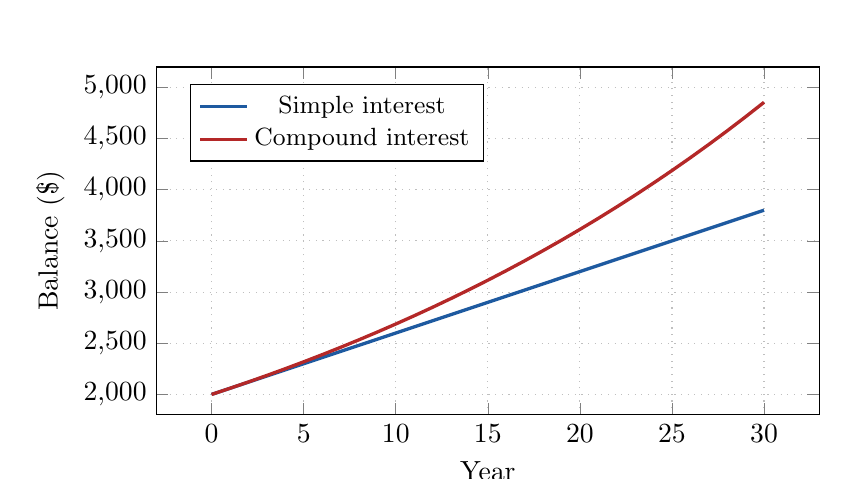
\begin{tikzpicture}
\begin{axis}[
  width=10cm, height=6cm,
  xlabel={Year},
  ylabel={Balance (\$)},
  xtick={0,5,10,15,20,25,30},
  ytick={2000,2500,3000,3500,4000,4500,5000},
  ymin=1800, ymax=5200,
  grid=major, grid style=dotted,
  legend style={at={(0.05,0.95)}, anchor=north west, font=\small},
]
\addplot[mathblue, very thick, mark=none,
  domain=0:30, samples=31]
  {2000*(1 + 0.03*x)};
\addlegendentry{Simple interest}
\addplot[mathred, very thick, mark=none,
  domain=0:30, samples=31]
  {2000*(1.03^x)};
\addlegendentry{Compound interest}
\end{axis}
\end{tikzpicture}
\end{center}
\end{example}

\subsection*{Compounding More Frequently}

Interest can be compounded more than once per year.
If interest is compounded $n$ times per year, each compounding
period uses the rate $\frac{r}{n}$, and there are $nt$
compounding periods in $t$ years.

\begin{definition}{General compound interest formula}
\[
A = P\!\left(1 + \frac{r}{n}\right)^{nt}
\]
where $n$ is the number of compounding periods per year.
\end{definition}

\begin{example}
\$1{,}000 at $6\%$ annual interest for 10 years under
different compounding frequencies.

\begin{center}
\renewcommand{\arraystretch}{1.5}
\begin{tabular}{lcc}
\toprule
\textbf{Compounding} & $n$ &
\textbf{Balance after 10 years} \\
\midrule
Annually    & 1   & \$1{,}790.85 \\
Semi-annually & 2 & \$1{,}806.11 \\
Quarterly   & 4   & \$1{,}814.40 \\
Monthly     & 12  & \$1{,}819.40 \\
Daily       & 365 & \$1{,}822.03 \\
\bottomrule
\end{tabular}
\end{center}

More frequent compounding produces a higher balance, but the
differences diminish as the frequency increases. The balance is
updated more often, and each percentage is applied to the latest state.
\end{example}

\begin{exercises}
  \item Compute the total amount $A$ for each situation.
    Round to the nearest cent.
    \begin{enumerate}[label=(\alph*), itemsep=4pt]
      \item $P = \$1{,}000$, $r = 5\%$, $t = 4$ years,
        compounded annually
      \item $P = \$500$, $r = 8\%$, $t = 3$ years,
        compounded annually
      \item $P = \$2{,}000$, $r = 4\%$, $t = 6$ years,
        compounded monthly
    \end{enumerate}

  \item An account starts with \$3{,}000 at $4\%$
    compounded annually.
    \begin{enumerate}[label=(\alph*), itemsep=4pt]
      \item Fill in the balance table for years 0 through 5
        by multiplying each year's balance by $1.04$.
      \item Compare the interest earned in year 1 with the
        interest earned in year 5.
        Explain the difference in one sentence.
    \end{enumerate}

  \item \$1{,}500 is invested at $6\%$ for 10 years.
    Compute the final balance under:
    \begin{enumerate}[label=(\alph*), itemsep=4pt]
      \item Simple interest
      \item Compound interest, compounded annually
      \item Compound interest, compounded monthly
    \end{enumerate}
    Rank the three results from smallest to largest.

  \item A savings account compounds monthly at an annual
    rate of $3\%$.
    What is the effective annual yield?
    Use the formula $A = P(1 + r/12)^{12}$ with $P = 1$
    and $t = 1$, and subtract $1$ from the result.
\end{exercises}

%--------------------------------------------------------------------
\section{The Rule of 72}
%--------------------------------------------------------------------

The Rule of 72 is an approximation for the doubling time
of a compound interest account.

\begin{definition}{Rule of 72}
At an annual compound interest rate of $r\%$, money
approximately doubles in:
\[
t \approx \frac{72}{r}\ \text{years.}
\]
\end{definition}

\noindent
The Rule of 72 applies equally to any quantity growing by
a fixed percentage per period: savings, debt, population,
or inflation. It gives a quick view of how a repeated multiplicative
update amplifies a starting state over time.

\begin{example}
\begin{enumerate}[label=(\alph*), itemsep=5pt]
  \item At $6\%$ annual interest, money doubles in
    approximately $72 \div 6 = 12$ years.

  \item At $9\%$, money doubles in approximately
    $72 \div 9 = 8$ years.

  \item A credit card charges $18\%$ annual interest.
    An unpaid balance doubles in approximately
    $72 \div 18 = 4$ years if no payments are made.

  \item Inflation at $3\%$ per year halves the purchasing
    power of money in approximately $72 \div 3 = 24$ years.
\end{enumerate}
\end{example}

\begin{example}[Verifying the Rule]
Using the compound interest formula to find the exact
doubling time at $6\%$:
\[
2P = P(1.06)^t \;\Rightarrow\; 2 = (1.06)^t.
\]
The exact solution requires logarithms and gives
$t \approx 11.9$ years.
The Rule of 72 gives $72/6 = 12$ years, a close approximation.
\end{example}

\begin{exercises}
  \item Use the Rule of 72 to estimate the doubling time
    for each interest rate.
    \begin{enumerate}[label=(\alph*), itemsep=4pt]
      \item $4\%$ \hfill
      \item $8\%$ \hfill
      \item $12\%$ \hfill
      \item $2\%$ \hfill
    \end{enumerate}

  \item A student loan has an interest rate of $6\%$.
    The student does not make payments for 12 years
    while in graduate school.
    \begin{enumerate}[label=(\alph*), itemsep=4pt]
      \item Use the Rule of 72 to estimate whether the
        loan balance has doubled after 12 years.
      \item If the original loan was \$30{,}000, estimate
        the balance after 12 years.
    \end{enumerate}

  \item If money doubles in 9 years under compound interest,
    what is the approximate annual interest rate?
    Set up the Rule of 72 equation and solve for $r$.

  \item An investment grows at $6\%$ per year.
    Using the Rule of 72, estimate how many years it takes
    to grow to four times its original value.
    \textit{Hint: four times means two doublings.}
\end{exercises}

%--------------------------------------------------------------------
\section{Loans}
%--------------------------------------------------------------------

A loan begins with a lender providing a principal $P$ to a
borrower.
Each period, two things happen.
\begin{enumerate}[itemsep=3pt]
  \item The outstanding balance increases by compound
    interest.
  \item The borrower makes a fixed payment that reduces
    the balance.
\end{enumerate}

\noindent
The monthly interest rate is $r_m = r_{\text{annual}} \div 12$.
The balance is updated by two competing effects: interest uses the
current balance and increases it; the scheduled payment is then
subtracted. If the payment is no larger than the interest charged,
the balance will not decrease.

\medskip
\noindent
The balance after each payment is computed as:
\[
B_{n+1}=B_n(1+r_m)-M,
\qquad
\text{new balance}=(\text{current balance})(1+r_m)-\text{payment}.
\]

\begin{example}
A \$4{,}000 loan at $6\%$ annual interest compounded monthly,
with fixed monthly payments of \$200.
Monthly interest rate: $r_m = 0.06 \div 12 = 0.005$.

\begin{center}
\renewcommand{\arraystretch}{1.6}
\begin{tabular}{cccc}
\toprule
\textbf{Month} & \textbf{Balance} &
\textbf{Interest} & \textbf{After payment} \\
\midrule
0 & \$4{,}000.00 & & \\
1 & \$4{,}000.00 & $+\$20.00$ & \$3{,}820.00 \\
2 & \$3{,}820.00 & $+\$19.10$ & \$3{,}639.10 \\
3 & \$3{,}639.10 & $+\$18.20$ & \$3{,}457.30 \\
4 & \$3{,}457.30 & $+\$17.29$ & \$3{,}274.59 \\
5 & \$3{,}274.59 & $+\$16.37$ & \$3{,}090.96 \\
\bottomrule
\end{tabular}
\end{center}

In month 1, \$20 of the \$200 payment goes to interest and
\$180 reduces the principal.
In month 5, only \$16.37 goes to interest, and \$183.63
reduces the principal.
As the balance falls, each payment retires a larger fraction
of principal.
\end{example}

\begin{example}[Total cost of a loan]
Continuing the loan from Example 6.4.1, 21 payments of
\$200 leave a balance of about \$24.87 before month 22.
After one more month of interest, the final payment is about
\$24.99. Therefore,
\[
\text{Total paid}=21(\$200)+\$24.99=\$4{,}224.99,
\]
\[
\text{Total interest}=\$4{,}224.99-\$4{,}000=\$224.99.
\]
The final payment is smaller than the regular payment because it
only needs to clear the remaining balance.

\begin{center}
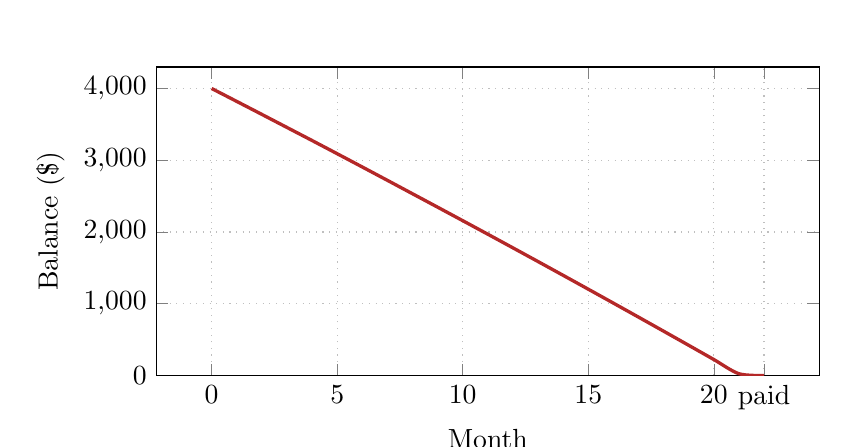
\begin{tikzpicture}
\begin{axis}[
  width=10cm, height=5.5cm,
  xlabel={Month},
  ylabel={Balance (\$)},
  xtick={0,5,10,15,20,22},
  xticklabels={0,5,10,15,20,paid},
  ymin=0, ymax=4300,
  grid=major, grid style=dotted,
]
\addplot[mathred, very thick, smooth]
  coordinates {
    (0,4000)(1,3820)(2,3639)(3,3457)(4,3275)
    (5,3091)(6,2906)(7,2720)(8,2533)(9,2346)
    (10,2158)(11,1969)(12,1779)(13,1588)
    (14,1396)(15,1203)(16,1009)(17,814)
    (18,618)(19,421)(20,223)(21,25)(22,0)};
\end{axis}
\end{tikzpicture}
\end{center}
\end{example}

\begin{example}[Effect of payment size]
The same \$4{,}000 loan at $6\%$ annual interest compounded
monthly, under different payment amounts. The final payment may be
smaller than the regular payment; totals below use cent-rounded
monthly interest.

\begin{center}
\renewcommand{\arraystretch}{1.5}
\begin{tabular}{cccc}
\toprule
\textbf{Monthly payment} & \textbf{Months to pay off} &
\textbf{Total paid} & \textbf{Total interest} \\
\midrule
\$150 & 29 & \$4{,}303.84 & \$303.84 \\
\$200 & 22 & \$4{,}224.99 & \$224.99 \\
\$300 & 14 & \$4{,}150.01 & \$150.01 \\
\bottomrule
\end{tabular}
\end{center}

Larger payments shorten the loan term and reduce total
interest paid.
\end{example}

\begin{exercises}
  \item A \$3{,}000 loan is charged $9\%$ annual interest
    compounded monthly.
    The monthly interest rate is $0.09 \div 12 = 0.0075$.
    The monthly payment is \$150.
    \begin{enumerate}[label=(\alph*), itemsep=4pt]
      \item Complete the loan table for the first four months.

      \begin{center}
      \renewcommand{\arraystretch}{1.7}
      \begin{tabular}{cccc}
      \toprule
      \textbf{Month} & \textbf{Balance} &
      \textbf{Interest} & \textbf{After payment} \\
      \midrule
      0 & \$3{,}000.00 & & \\
      1 & \$3{,}000.00 & $\$3{,}000 \times 0.0075 =$ & \\
      2 & & & \\
      3 & & & \\
      4 & & & \\
      \bottomrule
      \end{tabular}
      \end{center}

      \item In month 1, how much of the \$150 payment
        goes toward interest, and how much toward
        reducing the principal?
    \end{enumerate}

  \item A car loan of \$12{,}000 at $4.8\%$ annual interest
    compounded monthly has a monthly payment of \$400.
    Monthly rate: $0.048 \div 12 = 0.004$.
    \begin{enumerate}[label=(\alph*), itemsep=4pt]
      \item Complete the loan table for the first three months.
      \item After the third payment, what fraction of the
        original principal has been repaid?
    \end{enumerate}

  \item A student owes \$8{,}000 on a credit card charging
    $18\%$ annual interest compounded monthly
    (monthly rate $= 0.015$).
    The minimum payment is \$160 per month.
    \begin{enumerate}[label=(\alph*), itemsep=4pt]
      \item Compute the interest charge in month 1.
      \item How much of the first payment reduces the
        principal?
      \item At this rate, explain in one sentence whether
        the minimum payment is sufficient to eventually
        pay off the debt.
    \end{enumerate}

  \item Explain in two complete sentences why the fraction
    of each payment going toward interest decreases over
    the life of a loan.
    Use the loan balance as part of your explanation.
\end{exercises}

%--------------------------------------------------------------------
\section{The Observer and the Loan}
%--------------------------------------------------------------------

A loan agreement contains a fixed set of numbers: principal,
interest rate, payment amount, and term.
The bank and the borrower extract different information from
those same numbers because they are asking different questions.

\begin{center}
\renewcommand{\arraystretch}{1.5}
\begin{tabular}{ll}
\toprule
\textbf{The bank asks} & \textbf{The borrower asks} \\
\midrule
What is the total interest collected? &
  What is my monthly payment? \\
What is the annual percentage yield? &
  How long until I am debt-free? \\
What is the default risk? &
  How much of each payment is interest? \\
What is the effective return on capital? &
  What does this loan cost in total? \\
\bottomrule
\end{tabular}
\end{center}

\noindent
The loan terms and balance remain the same; the bank and borrower
choose different quantities to calculate because they are asking
different questions. The shared information can support several
perspectives, and each perspective selects a different feature to
interpret.

\medskip
\noindent
This structure also appears in the comparison between simple
and compound interest.
An observer asking ``what is the balance after one year?''
gets the same answer from both models at a $3\%$ rate
(both earn \$60 on a \$2{,}000 principal in year one).
An observer asking ``what is the balance after 30 years?''
gets very different answers.
The question determines when the distinction matters.

\begin{example}
A borrower takes a \$10{,}000 loan at $5\%$ annual interest
compounded monthly. The regular monthly payment is \$230.30 for
47 months, followed by a final payment of about \$229.96 in month 48.

The bank's perspective:
\begin{itemize}[itemsep=3pt]
  \item Total collected: $47 \times \$230.30 + \$229.96 = \$11{,}054.06$.
  \item Total interest: $\$11{,}054.06 - \$10{,}000 = \$1{,}054.06$.
  \item Total interest is about $10.54\%$ of the original principal over 4 years.
\end{itemize}

The borrower's perspective:
\begin{itemize}[itemsep=3pt]
  \item The scheduled payment is about \$230.30 per month.
  \item The loan is retired in 48 months.
  \item Total cost above principal is \$1{,}054.06.
\end{itemize}
\end{example}

\begin{exercises}
  \item A \$6{,}000 loan at $7.2\%$ annual interest compounded
    monthly has a regular payment of \$185.82 for 35 months and a
    smaller final payment in month 36.
    \begin{enumerate}[label=(\alph*), itemsep=4pt]
      \item Compute the total amount paid.
      \item Compute the total interest paid.
      \item Write one sentence describing this loan from
        the borrower's perspective.
      \item Write one sentence describing this loan from
        the lender's perspective.
    \end{enumerate}

  \item Two loans both have a principal of \$5{,}000 and an
    annual rate of $6\%$ compounded monthly.
    Loan A has monthly payments of \$150.
    Loan B has monthly payments of \$250.
    \begin{enumerate}[label=(\alph*), itemsep=4pt]
      \item Without completing full tables, predict which
        loan will cost more in total interest.
        Explain in one sentence.
      \item Compute the first month's interest charge for
        each loan.
      \item Explain why both loans have the same first
        month interest charge despite different payments.
    \end{enumerate}
\end{exercises}

%--------------------------------------------------------------------
\section*{Chapter 6 Review}
%--------------------------------------------------------------------

\addcontentsline{toc}{section}{Chapter 6 Review}

\begin{enumerate}[itemsep=8pt,leftmargin=2em]

  \item A \$5{,}000 investment earns $4\%$ simple interest
    per year.
    \begin{enumerate}[label=(\alph*), itemsep=4pt]
      \item Write the balance at year $t$ as a formula.
      \item Fill in the balance for years 0 through 5.
      \item How many years until the balance reaches
        \$6{,}000?
    \end{enumerate}

  \item The same \$5{,}000 investment earns $4\%$ compound
    interest per year.
    \begin{enumerate}[label=(\alph*), itemsep=4pt]
      \item Fill in the balance for years 0 through 5 by
        multiplying each year by $1.04$.
      \item Compare the interest earned in year 1 and
        year 5.
      \item How much more does the compound account hold
        after 5 years than the simple interest account?
    \end{enumerate}

  \item Use the Rule of 72 for each situation.
    \begin{enumerate}[label=(\alph*), itemsep=4pt]
      \item At what annual rate does money double in
        approximately 6 years?
      \item A retirement account earns $7\%$ per year.
        Approximately when will it double?
        When will it quadruple?
    \end{enumerate}

  \item A \$2{,}500 loan at $12\%$ annual interest
    compounded monthly (monthly rate $= 0.01$) has
    monthly payments of \$120.
    \begin{enumerate}[label=(\alph*), itemsep=4pt]
      \item Complete the loan table for months 1 through 4.
      \item How much of the month-1 payment reduces the
        principal?
      \item Estimate how many months the loan will take
        to pay off if the balance decreases by roughly
        \$95 per month on average.
    \end{enumerate}

  \item A credit card charges $24\%$ annual interest
    compounded monthly (monthly rate $= 0.02$).
    A balance of \$3{,}000 accrues with no payments made.
    \begin{enumerate}[label=(\alph*), itemsep=4pt]
      \item Use the Rule of 72 to estimate how many years
        until the balance doubles.
      \item Compute the balance after 12 months using the
        compound interest formula.
        Does this match the Rule of 72 estimate?
    \end{enumerate}

  \item Two accounts each start with \$1{,}000.
    Account A earns $5\%$ simple interest.
    Account B earns $4\%$ compounded annually.
    \begin{enumerate}[label=(\alph*), itemsep=4pt]
      \item Fill in balances for both accounts at years
        5, 10, 20, and 30.
      \item At what approximate year does Account B
        overtake Account A?
      \item Explain in two sentences why the compound
        account eventually exceeds the simple account,
        even though it has a lower interest rate.
    \end{enumerate}

  \item A homebuyer takes a mortgage of \$200{,}000 at $4.5\%$
    annual interest compounded monthly. It is to be repaid
    over 30 years with monthly payments of \$1{,}013.37.
    \begin{enumerate}[label=(\alph*), itemsep=4pt]
      \item Compute the total amount paid over 30 years.
      \item Compute the total interest paid.
      \item Express the total interest as a percentage
        of the original loan amount.
      \item Write two sentences: one from the borrower's
        perspective and one from the bank's perspective
        on this mortgage.
    \end{enumerate}

\end{enumerate}

\end{document}
